\chapter{CodeIgniter framework}
\paragraph{}

\paragraph{}
CodeIgniter is an Application Development Framework - a toolkit - for people who build web sites using PHP  \cite{codeigniter}. One of it's goals is to provide exceptional performance of web applications along with minimum complexity and fast development. CodeIgniter was born from ExpressionEngine \cite{elislab} in 2006 and since then, it increasingly gained popularity among PHP developers. In 2008 CodeIginiter became industry leader in an enviroment saturated with PHP frameworks \cite{elislab} and in 2014 CodeIgniter v 2.2 was released.

\paragraph{}
This framework is licensed under custom Elislab license, which is basicaly an open source license with only a few restrictions \cite{elislablicense}. We provide a copy of this license in medium attached to this work.

\paragraph{}
In this chapter, we will present a short guide of CodeIgniter request and response processing. Full user-guide and documentation can be found on CodeIgniter official website \cite{codeigniter}.

\section{Request and response flow}

\begin{figure}[h]
    \centering
    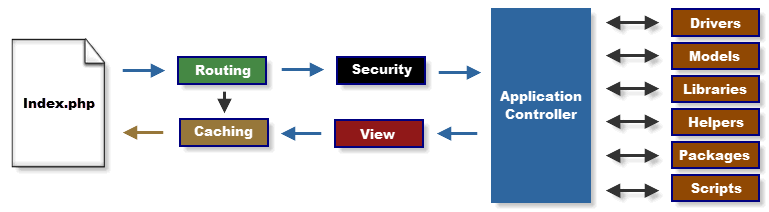
\includegraphics[width=0.85\textwidth]{images/codeigniter.png}
    \caption{CodeIgniter request flow}
    \label{codeigniter_flow}
\end{figure}

\paragraph{}
To understand how CodeIgniter works, let's look at processing of HTTP requests in this framework. CodeIgniter uses Apache2  module \texttt{mod rewrite}. This allows to be firstly processed \texttt{index.php} file as seen on image \ref{codeigniter_flow}. Purpose of this script is to load configuration of whole application, load routes, cache and other classes. It is provided by CodeIgniter framework and should not be changed (only for configuration purposes).

\paragraph{}
To process HTTP request, router must decide correct operation over it. If a cache file exists, it is sent directly to the browser, bypassing the normal system execution \cite{codeigniter}. Before the application controller is loaded, the HTTP request and any user submitted data is filtered for security.

\paragraph{}
In the next step, routing takes place. Each module of application must have it's own routes defined as follows:

\begin{lstlisting}[basicstyle=\small,caption={CodeIgniter routing}]
$route[course/(:num)] = "courses/$1";
\end{lstlisting}

\paragraph{}
The application takes list of all routes and applies the one of which regexp pattern matches the request URL. After this operation, proper controller (that must extend \texttt{CI\_ CONTROLLER} class) is selected, instanciated and method \texttt{run()} of this controller is run.

\paragraph{}
This controller loads data from models, can perform some operations over them and then data are sent directly to view. The finalized View is rendered then sent to the web browser to be seen. If caching is enabled, the view is cached first so that on subsequent requests it can be served instantly.

\section{Configuration and loading}
\paragraph{}
CodeIgniter also adds support configuration classes. These classes are located in \texttt{application/config} folder with possibility of creating multiple application enviroments. We have defined three of these enviroments, each for a different purpose: development(\texttt{localhost}), test (\texttt{devcourses.matfyz.sk}) and production (\texttt{courses.matfyz.sk}) . In this configs, all settings for database access, Oauth, PHP interpreter and other enviroment dependent variables must be located. 

\begin{lstlisting}[basicstyle=\small,caption={Database configuration for development enviroment}]
$db['default']['hostname'] = 'localhost';
$db['default']['username'] = 'root';
$db['default']['password'] = 'root';
$db['default']['database'] = 'courses';
$db['default']['dbdriver'] = 'mysql';
$db['default']['dbprefix'] = '';
\end{lstlisting}

\paragraph{}
Another important feature of CodeIgniter is autolading of resources. Major drawback of development in PHP is that application must be instantiated, interpreted and run each time for every request. For optimalization purposes, we do not want each time to instantiate all of the application classes, just the ones we need. Also, it is often annoying to import many classes in controllers or models. Elegant solution for these problems is resource autoloading, which is provided as a CodeIgniter core functionality. In \texttt{config/autoload.php} we can specify all classes or paths we want to autoload and CodeIgniter will import them when application needs them.


\section{Demonstration of Model-View-Controller}
Now that we have enough knowledge of CodeIgniter background processing, we can focus on development. In this section, we will provide examples and demonstrate development in this framework.

\subsection{Model}
\paragraph{}
We cannot start explaining models without writing about active records. CodeIgniter uses a modified version of the Active Record Database Pattern. This pattern allows information to be retrieved, inserted, and updated in your database with minimal scripting. In some cases only one or two lines of code are necessary to perform a database action. CodeIgniter does not require that each database table be its own class file. It instead provides a more simplified interface. \cite{codeigniter} This interface might seem similar to many ORM mappers.

\begin{lstlisting}[label={model}, caption={Article model}]
class Article_model extends CI_Model
{

    function __construct()
    {
        parent::__construct();
    }

    function get_article($id)
    {
        return $this->db->from('article')
            ->where('id', $id)
            ->get()
            ->result_row();
    }
}
\end{lstlisting}


\paragraph{}
As we can see on listing \ref{model}, each model has to extend \texttt{CI\_Model} class, which is the base class for each model and provides active records functionality. We also can not forget to call \texttt{parent::\_\_construct()} in our constructor.

\paragraph{}
This is just an example of very simplified model, whose only purpose is to load one article with specified \texttt{id} from database. This file should be located in folder \texttt{application/models} and named \texttt{article\_model.php}.   Now, let's focus on views.

\subsection{View}

\begin{lstlisting}[label={view}, caption={Article view}]
<html>
	<head>
		<title>Article page</title>
	</head>
	<body>
		<h1>Article says:</h1>
		<div>
			<?php $article->content ?>
		</div>
	</body>
</html>
\end{lstlisting}

\paragraph{}
All views are placed in \texttt{application/views} folder. Views are mostly HTML files with some PHP formatting code. We do not put any logic inside views. As we said, this view is just HTML with one PHP variable inside. How can we fill this variable? This is the time, when controller steps in.

\subsection{Controller}
Controllers must extend \texttt{CI\_CONTROLLER} class. It is a base class which provides basic functionality for application management, such as view and models loading, routing or request/response management. To put our example to work, we have to write a controller like this:

\begin{lstlisting}[label={controller}, caption={Article controller}]
<?php

class Article extends MY_Controller
{
    function __construct()
    {
        parent::__construct();
    }

    function show()
    {
    		$id = $this->uri->segment(3);
    		$article = $this->article_model->get_article($id);
    		$this->layout->set_content('views/article_view', array('article' => $article);
    }
}
\end{lstlisting}

\paragraph{}
Now, let's explain what we did in listing \ref{controller}. At first, we had to make a \texttt{\_\_construct} method with \texttt{parent} call. This will instantiate controller basic functionality. In method called \texttt{show()} we at first got an ID of article. This ID comes from accessed URL. Full URL route to this controller would be \texttt{domain.com/article/show/:id}, where \texttt{:id} serves as specified ID. In the next step we used call from our model, which is autoloaded and then we filled this data to our view. And voila, building applications with CodeIgniter is simple!

